\section{Introduction}
\label{sec:intro}
%Traffic problems pose much pressure on urban planning. Nowadays, 
%as the number of vehicles in cities explodes, traffic jams and 
%accidents becomes commonplace, which is both time-consuming and inconvenient. 
%Thus, it would be extremely useful if there exists a system that
%predicts the urban traffic conditions under different settings. 
%First of all, it can help urban planners optimize roads and arrange land usage for traffic, \figref{fig:urban1} and \figref{fig:urban2} show a typical example. Governments can forecast whether the construction of a new road 
%can ease the traffic. Property developer can assess whether building a 
%new shopping mall will cause congestion. This help urban planner make 
%better, more informed decisions. Second, predicting the traffic at
%future time can help users better organize their itinerary and routes. 
%Users only need to input time, then they can get the traffic condition 
%along the intended route, which is allows users to make alternate plans
%in advance. Finally, the technique can help with the transport distribution. 
%For instance, if companies such as Uber use our product, 
%they can distribute their vehicle resources in a more optimized manner, 
%resulting in more passengers without causing traffic jam, 
%this will benefit both passengers and the companies.

%\begin{figure}[th]
%    \centering
%	\begin{subfigure}[t]{0.49\columnwidth}
%	\resizebox{\columnwidth}{!}{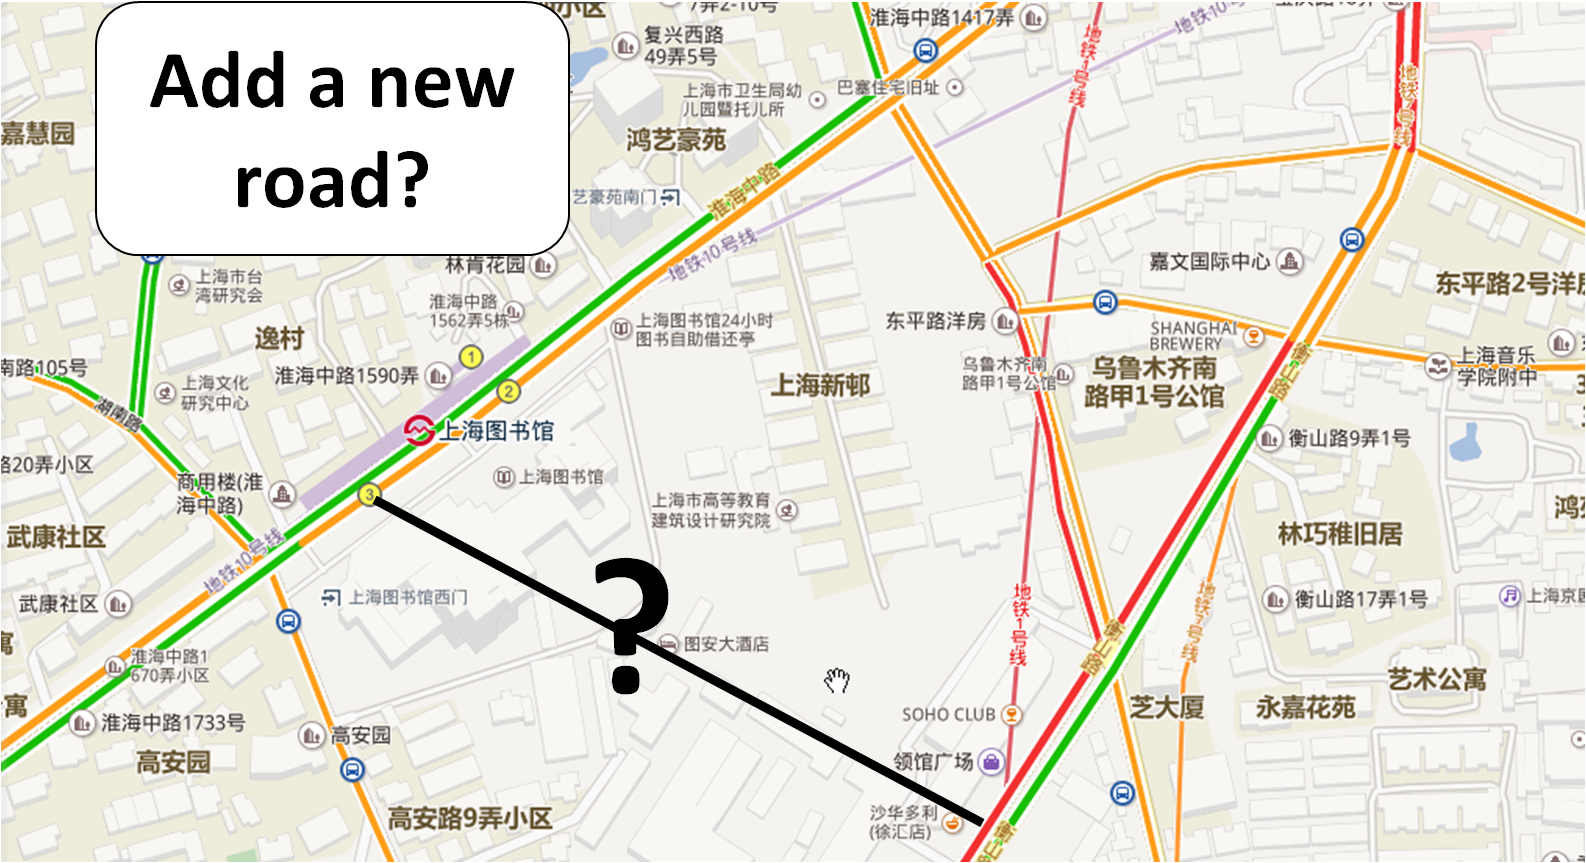
\includegraphics{figures/data/urban1.png}}
%	\caption{before construction}
%	\label{fig:urban1}
%	\end{subfigure}
%	\begin{subfigure}[t]{0.49\columnwidth}
%	\resizebox{\columnwidth}{!}{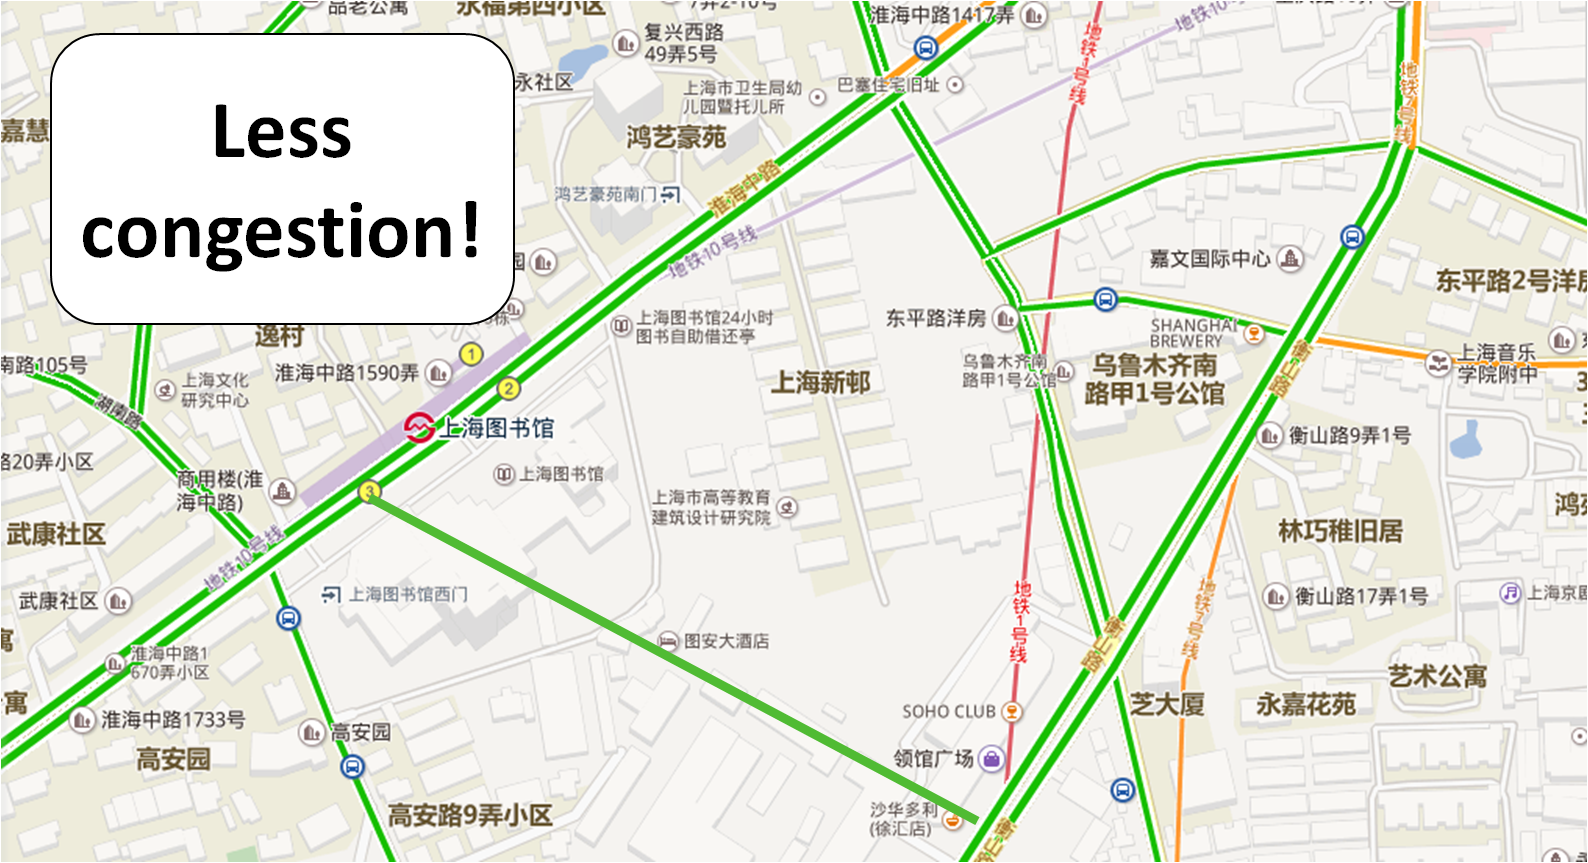
\includegraphics{figures/data/urban2.png}}
%	\caption{after construction}
%	\label{fig:urban2}
%	\end{subfigure}
%	\caption{using prediction model on urban planning}
%\end{figure}

The goal of this work is to develop a framework and a system to 
predict traffic conditions on any roads given a map formatted in 
OpenStreetMap data~\cite{openstreetmap}. 
Traffic prediction can help urban planners optimize roads and arrange land usage. Also, it can assist people to organize their itinerary and routes more reasonable. In addition, it can help with transport distribution. The inputs to the problem include: 
the topological map data, time of the day, day of the week, 
location and weather, etc. The output will be classified 
into four classes: green (good), yellow (slow), red (congested) 
and deep red (extremely congested). 

There are four major challenges in this research. 
The first one is the data incompleteness. 
Baidu Map does not directly share their data of POIs and real-time traffic information. Although OpenStreetMap is free, it lacks lots of POIs in China and 
has no real-time traffic information. 
Apart from that, integrating these two resources is also difficult because the two maps are using different coordinate systems.
The third challenge is feature selection. There are plenty of features 
that will influence the traffic conditions. We need to select all the 
possible features without introducing noises. 
The last one
is the data imbalance. This dataset is predominately composed
of green (good) than other classes.

Our approach can be divided into three stages.
\begin{itemize}
\item First, integrating
the map data and live traffic data from Baidu Map into OSM. 

\item Second, feature engineering. In this stage, we come up with many useful features.

\item Third, prediction model training.
We use multi-class linear SVM with weight~\cite{multisvm} to train our model.

\end{itemize}
%So we train a fixed size three-level binary decision tree of weighted SVM classifiers.
%Each binary classifier is trained from data which is modified by SMOTE, combining oversampling and under-sampling.
%Our alogrithm combines multi-class linear SVM with SMOTE to increase our accuracy, which solve the problem of imbalanced data.

%combining binary decision tree with weighted SVM  
%algorithm, so we can get a proper prediction model to predict 
%traffic in the future.

%We will produce a web demo which is efficient and user friendly. We shall dig into various types of machine learning and data mining models, as well as simulation methods, mostly focusing on spatial-temporal data. By comparing those methods and fine-tuning the parameters, we would conclude the combinations that our system uses and reveal insights on the principle of how population move in urban areas. Also, as an engineering project, a system and a demo with interactive functionality that may be able to be put into industry is crucial.

The main contributions of this paper are as follows:
\begin{itemize}
\item First, our system can do cross prediction, we employ the transfer learning concept
in traffic prediction field so that we can predict traffic in areas where we do not have any historical traffic data, which is one of the first systems that are enable to do this.

%Traditional machine learning are based on the assumption that training and future data
%in the same space and have same distribution. But in real-world, many cases are that we have training data in one domain while 
%testing data in another domain. Our model can solve this problems in traffic prediction. For example, in Shanghai, we can use the data 
%in each district to predict traffic in other districts with high accuracy.


%We combine binary decision
%tree model with weighted SVM. Data imbalance is a serious problem for real-world issue since 
%real-world datasets are predominately composed of normal examples with only a small percentage of abnormal examples.
%Thus, the training tend to classify data into normal cases. As our
%problem is multi-class which makes it even harder.



%=======
%\item Second, our approach to solve the data imbalance problem is effective. We combine binary decision
%tree model with weighted SVM. 
%Data imbalance is a serious problem for real-world issue since 
%real-world datasets are predominately composed of normal examples with only a small percentage of abnormal examples.
%Thus, the training tend to classify data into normal cases. As our
%problem is multi-class which makes it even harder.
%Our first model is a multi-class SVM with weights. This naive model is far from satisfaction.
%Then we optimize this model by binary decision tree model where each node is a binary
%SVM trained from data rebalanced with SMOTE \cite{chawla2002smote} or simply by SVM with miss-classification penalty.
%Our experiment results show that binary decision tree with weighted SVM perform the best.
%So we build our model by combining decision tree with weighted SVM.

%So we train a fixed size three-level binary decision tree of weighted SVM classifiers.
%Each binary classifier is trained from data which is modified by SMOTE, combining oversampling and under-sampling.
%Our alogrithm combines multi-class linear SVM with SMOTE to increase our accuracy, which solve the problem of imbalanced data.

\item Second, our system combines diverse useful features that can be categorized into two types: geospatial features and implicit features. 

\item Third, our approach to address the data imbalance issue is effective in this particular multi-classification problem. 
%In China, we can acquire real-time traffic information only by Baidu Map.
%Baidu's prediction are mainly based on time-series, while our prediction features are much more complete.
%In our features, \KZ{add some useful features here} are quite essential.More features provide us with more comprehensive model that can predict traffic
%condition accurately. 

%\item Fourth, our prediction results are much more accurate than Baidu and also can achieve cross prediction.
%This is mainly because the above three contributions. 
%With more features to optimize the model 
%and using binary decision tree algorithm together with weighted SVM, we solve the problem of imbalanced data. So 
%our model is much more reliable.
\end{itemize}
